\section{Model checking in \emph{Reprotool}.}

\subsection{Introduction to model checking in \emph{Reprotool}}.

\emph{Reprotool} project can contain many use-cases. Use-cases consist of use-case steps. You can assign annotaions to individual
use-case steps. These annotations are basicly boolean variables. When the \emph{Reprotool} performs model checking, it firstly
initializes all annotaion variables to boolean value false. It then starts executing use-cases. Executing a use-case means executing
its use-case steps. If a step with an annotation is being executed, the value of the corresponding  annotation variable is changed to true.
The annotaions in a \emph{Reprotool} project must adhere to the rules that are defined in the project as a set of temporal logic
formulas. When you run the model checking in \emph{Reprotool}, you are actually checking the validity of these temporal logic formulas.
By assigning new annotaions to use-case steps in the project, you are actually extending the set of logic formulas that will be verified
during the model checking process.

\subsection{Predefined \emph{Reprotool} annotaions an their semantics.}
In every \emph{Reprotool} project, there is already a set of predefined annotations that you can use. You can, however, define new
annotations and define their behaviour. The predefined annotations already have some predefined default behaviour.

\subsubsection {The \emph{open} and \emph{close} annotaions are bound by these rules:}

\begin{enumerate}
  \item After 'open' there should always be 'close'.
  \item No multi-open without close.
  \item No multi-close without open.
  \item First 'open' then 'close'.
\end{enumerate}

\subsubsection{The \emph{create} and \emph{use} annotaions are bound by these rules:}

\begin{enumerate}
  \item After 'create' there must be some branch containing 'use'.
  \item Only one 'create'.
  \item First 'create' then 'use'.
\end{enumerate}

\subsubsection{The special \emph{trace} and \emph{on} annotations}
These two annotations are special, you can not override their meaning. By using these annotations, you can conditionally prune the
execution tree of the model checker during the verification process. You will better understand their meaning when we demonstrate
their usage later in this chapter.

\subsection{Generating the NuSMV model}
To generate the \emph{NuSMV} model specification of the \emph{cityMap.swproj} project, right-click the file in the project explorer
and run the command \emph{Convert SW project to SMV}. Notice in the project explorer, that a new file \emph{cityMap.swproj.nusmv} has
been generated in the \emph{Citymap example} project directory. This file contains the model specification for the \emph{NuSMV} model checker.

Open the \emph{cityMap.swproj.nusmv} file. The file will be opened by our \mbox{\emph{NuSMVLang}} editor. Using this editor, it is possible to manualy edit the generated model.
There is a \emph{NuSMV Manual} in the documentation directory of the \emph{Reprotool} svn tree. Direct editing of this
file should however not be necessary.

\hyphenation{Ve-ri-fi-ca-tion}

\subsection{Model checking}
To run the \emph{NuSMV} verification for the generated model \emph{cityMap.swproj.nusmv}, right-click this file in the project explorer
and run the command \emph{Run NuSMV Verification} from the context menu. The \emph{NuSMV} model checker now finds a violation of one of
the temporal logic formulas specified for this project and prints into the console the counter-example trace. This trace consists of
a series of state transitions as defined in the \emph{NuSMV} model file \emph{cityMap.swproj.nusmv} that leads to the violation.
A human-readable form of this trace is also generated. Notice the file \emph{cityMap.swproj.cexmp} that has been generated in the project
directory.

\subsection{Reading the counter-example trace}
Open the generated counter-example trace in the file \emph{cityMap.swproj.cexmp}. You should see a screen similar to this:

\newpage

\begin{figure}[ht]
  \centering
  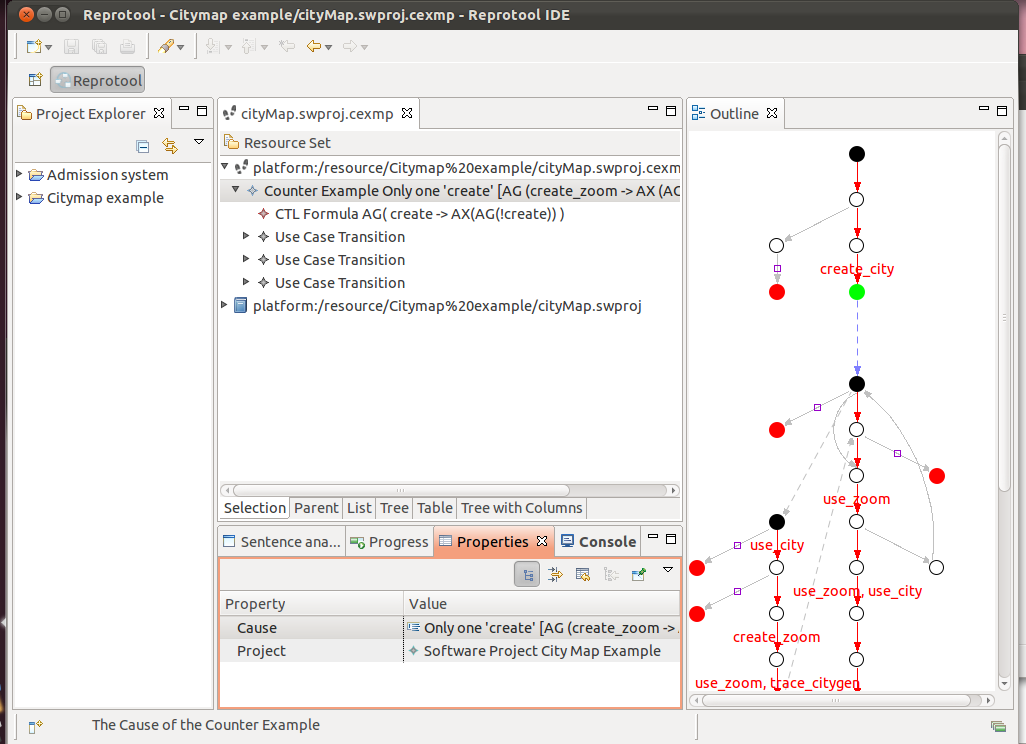
\includegraphics[height=280pt]{images/reprotoolTraceCityMap}
  \caption{Counter-example trace of the cityMap project}
  \label{fig:reprotoolTraceCityMap}
\end{figure}

Make sure that the outline and the properties views are visible. You can see the visual representation of the execution path in the
outline view. What we are going to find out by inspecting this trace is the temporal property that has been violated.
Click on the root \emph{Counter Example} tree node in the editor view that shows the counter-example trace. In the properties view,
you can see the \emph{Project} property that tells us for which project the counter-example has been generated. There is also the
\emph{Cuase} property that reads:
\begin{verbatim}
Only one 'create' [AG (create_zoom -> AX (AG !create_zoom)) ]
\end{verbatim}
This line contains the temporal logic formula description and then the actual formula in the square brackets. From the formula
description, we see that the problem is that some object has been created more than once. And from the actual formula, we can
see that the \emph{zoom} object is the one that has been created more than once. Now look carefully into the outline view and
follow the red line that shows us the execution path. You will see, that indeed the \emph{create\_zoom} annotaion appears two times
in the trace. And this causes the violation of the shown temporal logic formula.